\section{Shafts and axles}

	The first thing to keep in mind while dimensioning/verifying a shaft/axles is to consider the \textbf{service factor} (as in table \ref{tab:servicefactor}), a coefficient that multiplies the actual loading conditions depending on the characteristic of the driven machine; it can be seen as a safety factor.
	
	\begin{table}[b]
		\centering
		\rule{0.8\linewidth}{1pt}
		\caption{service factor in respect of the characteristic of the driven machine.}
		\label{tab:servicefactor}
		\begin{tabular}{ r | M{4cm}  M{4cm} }
			& Normal torque & High torque and/or non uniform working \\ \hline
			Uniform functioning &  1.0-1-1 &  1.2-1-3 \\
			Light impact & 1.2-1.3 & 1.3-1.4 \\
			Moderate impact & 1.4-1.5 & 1.5-1.6 \\
			High impact & 1.5-1.6 & 1.6-1.8
		\end{tabular}
		\rule{0.8\linewidth}{1pt}
	\end{table}

	For the design/verification we usually start off with a static/stress verification, then a stiffness one (to avoid high deflection) and then critical flexural speed and torsional oscillations. For shaft usually only the torsional and bending loads are considered due to their predominance.
	
	\paragraph{Preliminary design} For a preliminary dimensioning on the shaft we can consider a full/hollow circular cross section (with diameter $d$) that, subjected to a torsional component $T$, leads to the following tangential stress component:
	\begin{equation}
		\tau = \frac T{J_p} \frac d 2
	\end{equation}
	To take into account also bending loads $M_b$ we can use a simplified approach by computing an equivalent bending moment $M_{b,eq}$ of the form
	\begin{equation}
		M_{b,eq} = \sqrt{M_b^2 + \alpha T^2} \qquad \qquad \textrm{where } \ \alpha = \begin{cases}
			0.25 \quad & T \textrm{ constant} \\
			0.75 \quad & T \textrm{ alternating} \\
		\end{cases}
	\end{equation}

	Given the \textbf{section modulus} $Z$ of the section (for the circular one $Z = \frac \pi {32} d^3$) we can compute the maximum stress state on the structure as
	\begin{equation}
		\seq = \frac{M_{b,eq}}{Z}
	\end{equation}
	Observing that the equivalent tension $\seq$ should always be less then an allowable value $\sall = \sigma_{ys}/\phi$, by inverting the previous formula for the case of a full circular section we can dimension the minimum diameter of the shaft as
	\begin{equation} \label{eq:shaft:dmin}
		\begin{split}
			d_{min} & \geq \sqrt[3]{\frac{32}{\pi} \frac{M_{b,eq}}{\sigma_{all}} } \quad \,\textrm{: bending,torsion} \\
			& \geq \sqrt[3]{\frac{16}{\pi} \frac{T}{\tau_{all}} } \qquad \textrm{: torsion} 
		\end{split}
	\end{equation}
	
	Note that the choice of the yielding strength of the material can improve only the stress response of the shaft, while deflections can be handled by choosing appropriate geometries of the cross section.
	
	\paragraph{Geometry definition} Known the minimum diameter on the shaft that bears a related load applied, when adding shoulders to the component we have to always keep in mind the following \textit{rules} to avoid the insurgence of unwanted stress concentrations:
	\[ 1.2 \leq \frac D d \leq 1.5 \qquad \qquad \textrm{and} \qquad \qquad 0.02 \leq \frac r d\leq 0.06 \]
	where $D,d$ are the diameters of the bigger/smaller cross sections and $r$ is the fillet radius (\textit{raggio di raccordo}). For the first iteration in the design phase the worst scenario should be used, and so $r/d = 0.02$, by looking at table \ref{tab:scf-firstiter}. Later on in the verification phase more complete graphs might be used (figure \ref{fig:stressconcentrationfactors}).
	
	
	\begin{table}[bt]
		\centering
		\rule{0.8\linewidth}{1pt}
		\caption{first iteration estimates for stress concentration factors $K_t$/$K_{ts}$ depending on the type of load.}
		\label{tab:scf-firstiter}
		\begin{tabular}{ r | c c c }
			& bending $K_t$ & torsional $K_{ts}$ & axial \\ \hline
			shoulder fillet - sharp ($r/d=0.02$) & 2.7 & 2.2. & 3.0 \\
			shoulder fillet - well rounded ($r/d=0.1$) & 1.7 & 1.5 & 1.9 \\
			end-mill keyseat ($r/d=0.02$) & 2.14  & 3.0 & - \\
			sled runner keyseat & 1.7 & - & - \\
			retaining ring groove & 5.0 & 3.0 & 5.0
		\end{tabular}
		\rule{0.8\linewidth}{1pt}
	\end{table}
	
	\begin{figure}[bht]
		\centering
		\begin{subfigure}{0.48\linewidth}
			\centering 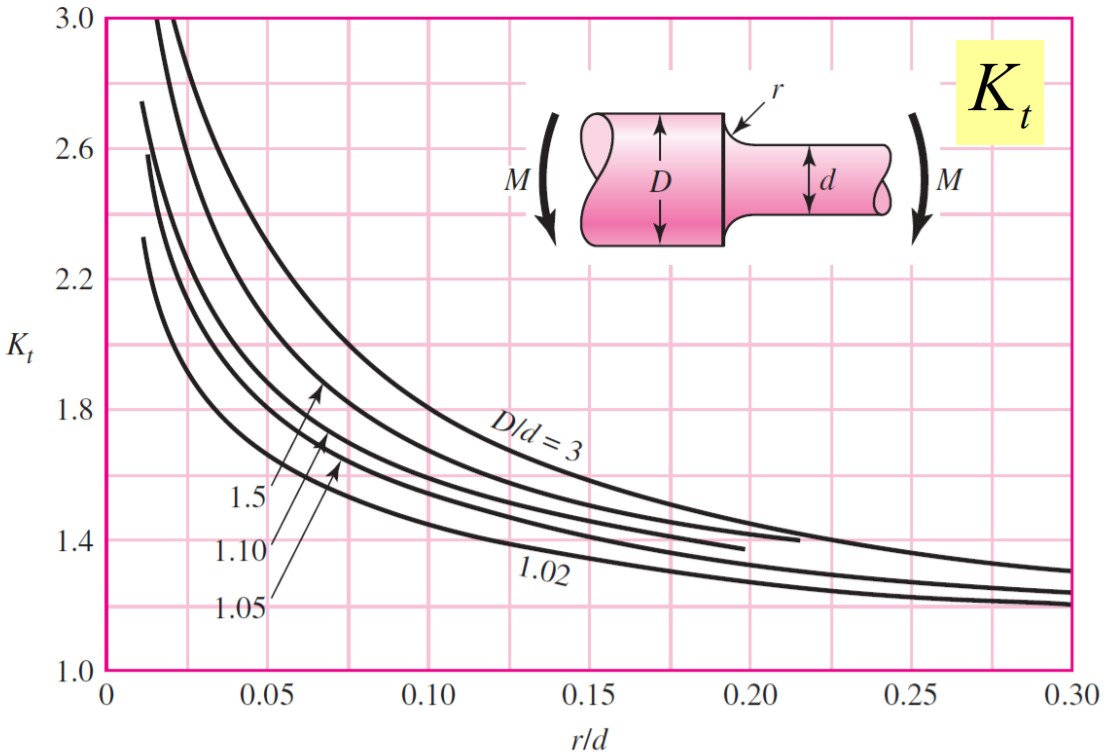
\includegraphics[width=\linewidth]{conc-factor-a} \caption{}
		\end{subfigure}
		\begin{subfigure}{0.48\linewidth}
			\centering 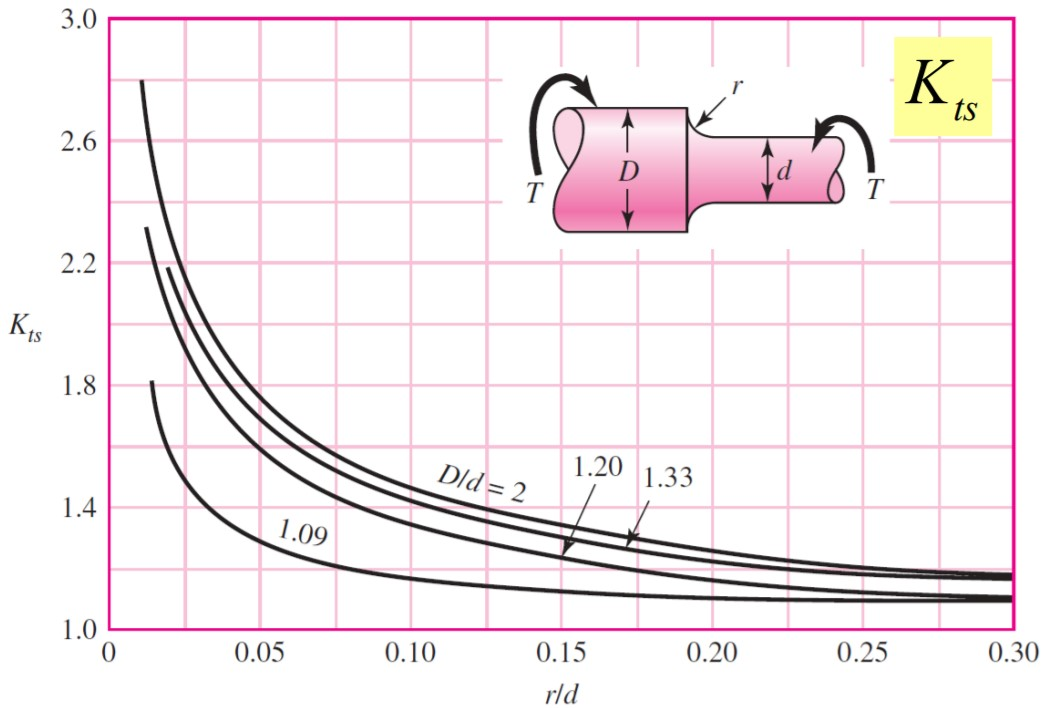
\includegraphics[width=\linewidth]{conc-factor-b} \caption{}
		\end{subfigure}
		\caption{stress concentration factors for bending $K_t$ (a) and torsional $K_{ts}$ (b) loads.} 
		\label{fig:stressconcentrationfactors}
	\end{figure}

	While doing a stiffness verification (using as example Castigliano's theorem) always keep in mind that usually bearings have a maximum angle of allowable deflection: having higher deflections leads to premature failure of the components. While computing deflections it's note necessary to take into account stress concentration factors because they don't have a \textit{high impact} in terms of displacement.
	
\subsection{Positive (geometric) coupling}
	
	\paragraph{Parallel keys}Given a parallel key (figure \ref{fig:parallelkey}) of length $L$ used to transmit a desirable torque $T$ between a shaft and a hub, we can assume the pressure $p$ on the sides of the key as uniformly distributed with value \[T \approx p(h-t) L \frac d 2\qquad \qquad \Rightarrow \qquad \qquad p \approx \frac{2T}{d(h-t)L}\]
	
	\begin{SCfigure}[2][bht]
		\centering 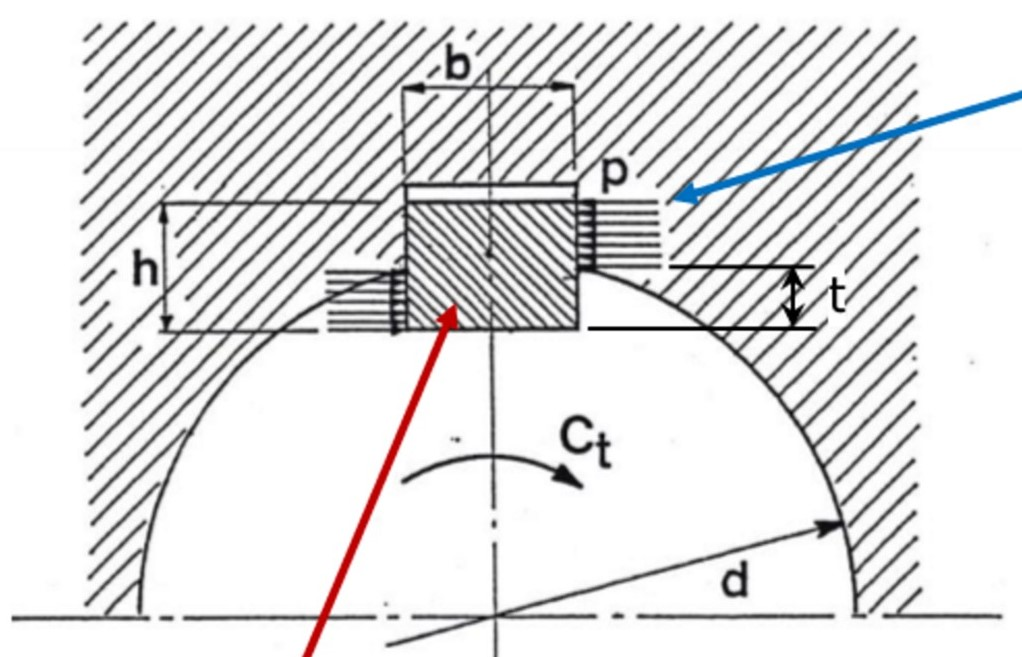
\includegraphics[width=5cm]{pos-coupling} 
		\caption{schematic representation of a geometric coupling made by a parallel key.} \label{fig:parallelkey}
	\end{SCfigure}
	
	In real application the dimensions of the key are determined by normative (such \texttt{UNI 6604}) where, given the diameter $d$ of the shaft, all the other dimension (such $b,h$) are set and only the length $L$ can be choose at will (depending on the pressure to bear), but as a rule of thumb we have that $L <1.5d$.
	
	To transmit more torque up to 3 keys can be mounted on the shaft determining a pressure $p$ that depends on the number $z$ of keys and a related \textbf{uniformity factor} $\phi$ (table \ref{tab:uniformityfactor}):
	\begin{equation}
		p\approx\frac{2T}{d(h-t)Lz\phi} \leq p_{all,hub}
	\end{equation}
		
	\begin{SCtable}[4][bht]
		\centering
		\begin{tabular}{c c}
			z & $\phi$ \\ \hline 1 & 1 \\ 2 & 0.75 \\ 3 & 0.67
		\end{tabular}		
		\caption{Uniformity factor $\phi$ depending on the number $z$ of parallel keys.}	\label{tab:uniformityfactor}
	\end{SCtable}
	
	While verifying such type of connection is important to consider the a stress concentration factor as shown in figure \ref{fig:stresskey}.
	
	\begin{figure}[bht]
		\centering 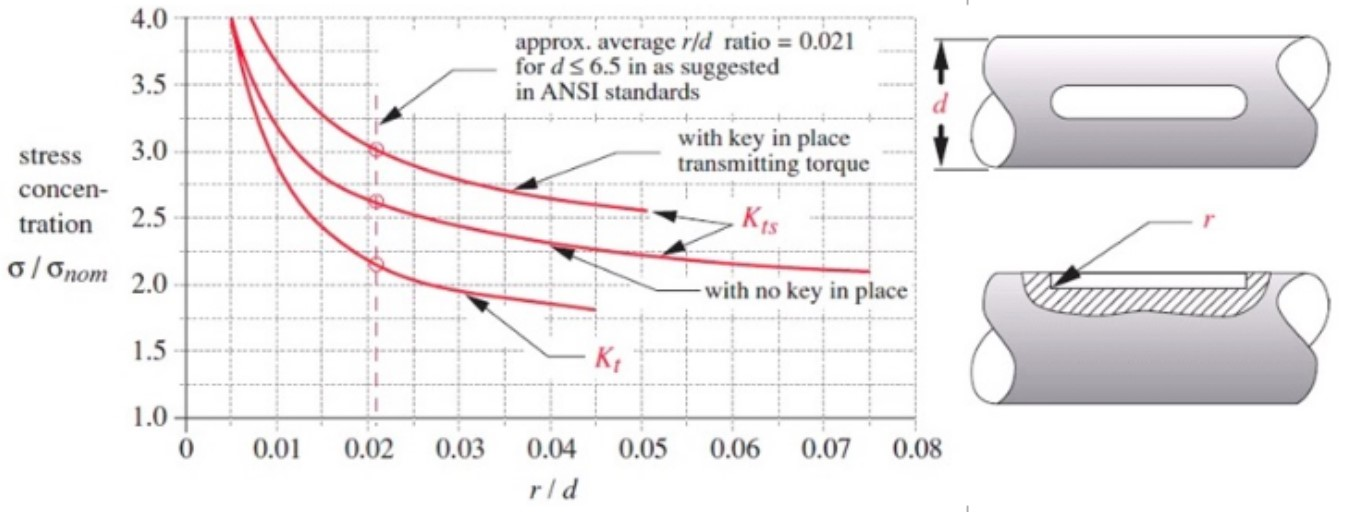
\includegraphics[width=0.8\linewidth]{stress-key} 
		\caption{stress concentration factor to use while dimension parallel keys.} \label{fig:stresskey}
	\end{figure}
	
	\paragraph{Splines} Positive coupling with splines (figure \ref{fig:spline}) is ideal when the torque to be transmitted is high; in this case the major drawback is the introduction of high notch effects that worsen the response to fatigue.
	
	\begin{SCfigure}[2] 
		\centering 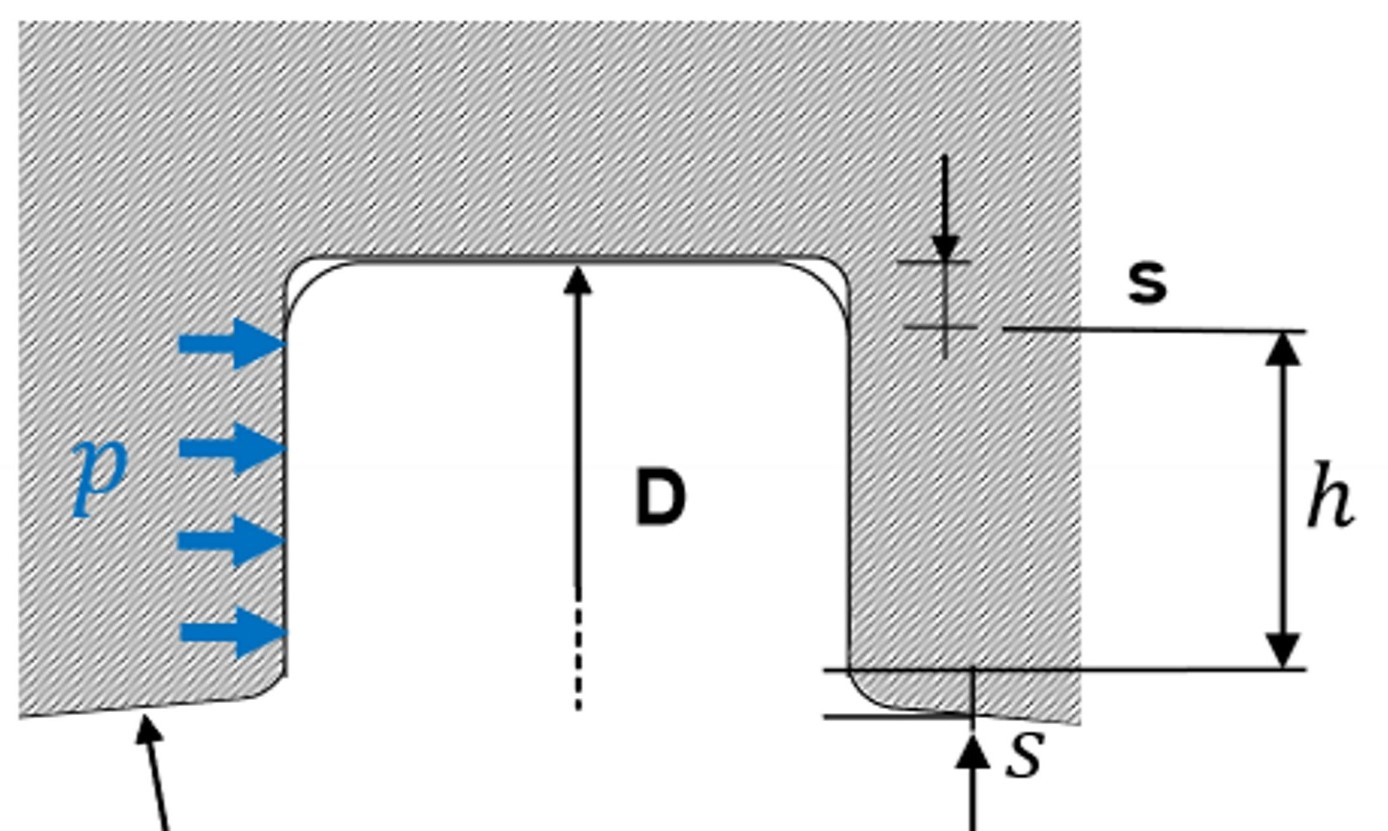
\includegraphics[width=4cm]{splines-dimensioning}
		\caption{scheme used for the design/verification of a spline positive connection.}
		\label{fig:spline}
	\end{SCfigure} 
	
	In order to dimension the spline we firstly need to determine the minimum shaft diameter $d$ in order to transmit the torque (from equation \ref{eq:shaft:dmin}), then outer diameter $D$ is automatically determined by normative (such \texttt{UNI 8953}) and, at last, we choose the minimum engagement length $L$ by making equally critical the shaft yielding and the spline profile bearing:
	\begin{equation}
		T_{max} = p_{all} h L \frac {d_m}2 z\psi = \tau_{all,shaft} \frac{\pi d^3}{16}
	\end{equation}
	where $d_m = \frac{D+d}{2}$ is the mean diameter, $z$ is the number of teeth and $\psi$ is the \textbf{load distribution factor} whose values are reporter in table \ref{tab:shaft:loaddistr}.
	
	\begin{table}[bht]
		\centering
		\rule{0.8\linewidth}{1pt}
		\caption{load distribution factor $\psi$ function of load type and contact surfaces.}
		\label{tab:shaft:loaddistr}		
		\begin{tabular}{M{4cm}  | M {3cm} M {3cm} }
			Contact surfaces & not sliding; sliding only when loaded & sliding when loaded \\ \hline
			both surfaces hardened & $\psi = 0.55$ & $\psi = 0.65$ \\
			no surfaces or one surface hardened & $\psi = 0.75$ & $\psi = 0.90$
		\end{tabular}
		\rule{0.8\linewidth}{1pt}
	\end{table}
	
\subsection{Friction coupling}
	
	\paragraph{Tapered press fit}In order to transmit torque using press fits connection (figure \ref{fig:pressfit}), the shaft has to present a conical section complementary to the hub's one defined by a conicity ratio
	\[ C = \frac{D-d}{L} = 2\tan \left( \frac \alpha 2\right)\]
	By analysing the contact forces exchanged between the shaft and the hub it's possible to compute the minimum pressure $p_{min}$ on the contact surface (that must always be smaller then an allowable threshold $p_{all}$) and so the torque $T$ transmitted as function of the axial force $F_a$ and the axial($f_a$)/torsional($f_t$) friction coefficients:
	\begin{equation}
		\begin{split}
			p_{min} & = \frac 4 \pi \frac{F_a \sin(\alpha/2)}{D^2-d^2}  \frac 1 {\sin(\alpha/2) + f_a\cos(\alpha/2)} \leq p_{all} \\
			T & = \frac 1 3  \frac{f_t F_a}{\sin(\alpha/2) + f_a\cos(\alpha/2)} \frac{D^3-d^3}{D^2-d^2}
		\end{split}
	\end{equation}
	
	\begin{figure}[bht]
		\centering
		\begin{subfigure}{0.48\linewidth}
			\centering 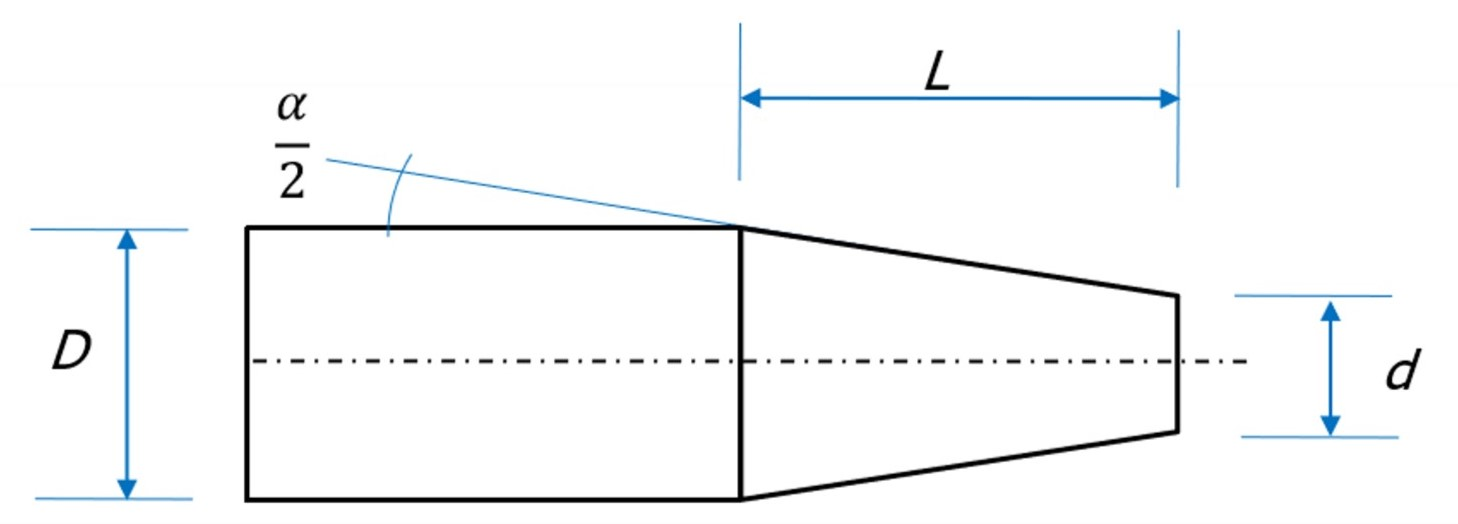
\includegraphics[width=0.9\linewidth]{pressfit-1} \caption{}
		\end{subfigure}
		\begin{subfigure}{0.48\linewidth}
			\centering 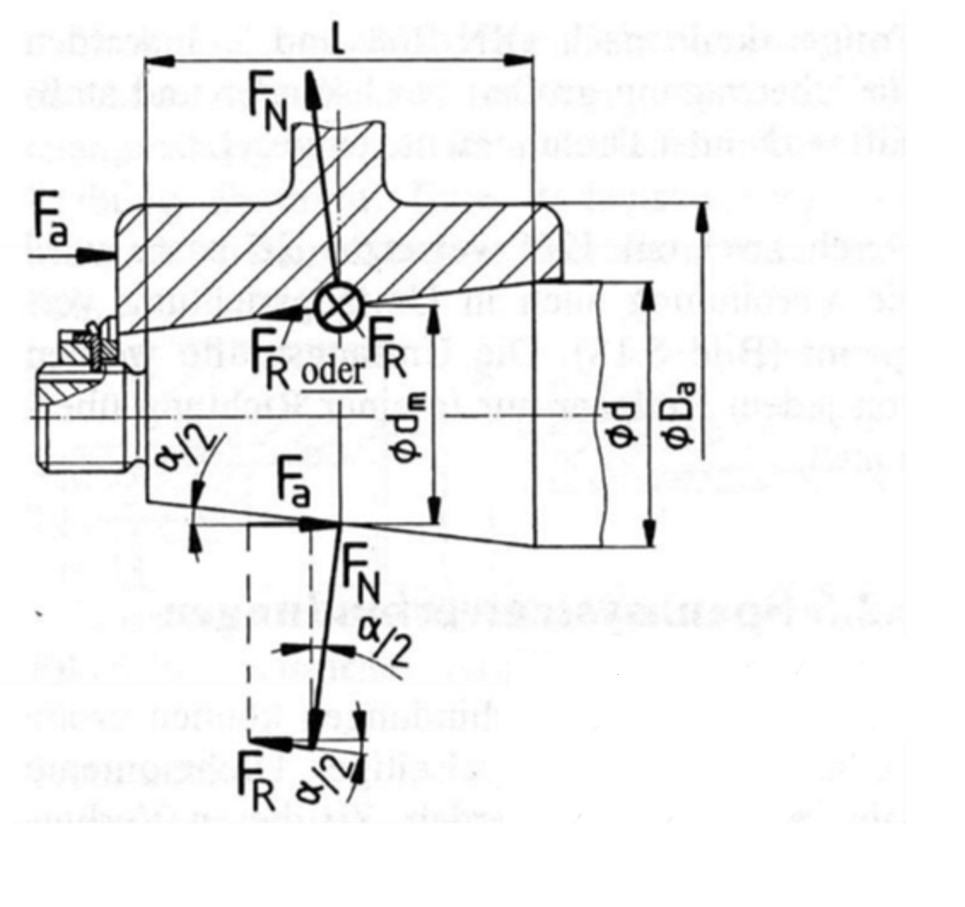
\includegraphics[width=6cm]{pressfit-2} \caption{}
		\end{subfigure}
		\caption{scheme to use while designing/verifying a tapered press fit connection.} \label{fig:pressfit}
	\end{figure}
	
	\subsubsection{Press (interference) fit} The interference $i$ between the dimension of the outer radius $r$ of a shaft and the inner radius $R$ of the hub has to have a minimum value $i_{min}$ in order to avoid the relative slipping of the two pieces, but also a maximum value $i_{max}$ in order to avoid yielding for the parts. 
	
	By  performing a full analyses we can see that the interference $i$ is linearly proportional to the contact pressure $p_c$ following the rule
	\begin{equation}
		i = p_c r_c \left( \frac 1 {E_2} \frac{R_o^2+r_c^2}{R_o^2-r_c^2} + \frac{\nu_2}{E_2} + \frac{1}{E_1}  \frac{r_c^2 + r_i^2}{r_c^2 - r_i^2} - \frac{\nu_1}{E_1}\right)
	\end{equation}
	where $r_c$ is the resulting radius of the circle after deformation of both hub and shaft; subscript 1 is associated to the inner part (the shaft) while subscript 2 is associated to the outer one (the hub). In the particular case of components made by the same material and a solid shaft, the expression reduces to
	\begin{equation} \label{eq:interferencesimple}
		i = 2 \frac{p_c r_c}{E} \frac 1 {1-\frac{r_c^2}{R_o^2}}
	\end{equation}
	In general, as good approximation, $r_c$ is considered as equal to $r_0$. To determine the minimum and maximum contact pressure and thus interference we need to consider both the action to transmit by the coupling and the yielding of the material:
	\begin{equation}
		p_{c,min} = \phi \frac \tau {f_t} = \frac{\phi}{f_t} \frac{\sqrt{\big(2 T/D\big)^2 + F_a^2}}{\pi DL} \qquad \qquad \qquad \qquad
		p_{c,max}  = \sigma_{eq} = \frac{\sigma_y}{\phi}
	\end{equation}
	To take into account the non-uniform distribution of the pressure due to the contact between shaft and hub, a stress concentration factor of at least $K_t = 2$ must be considered in the verification process of the structure. In general while designing a product we have to specify the diametral tolerance $\delta$ defined as $2i$ determined by the range $[\delta_{min},\delta_{max}]$ due to $p_{c,min}, p_{c,max}$; in table \ref{tab:metricfits} a table including tolerances for hole-base coupling has been presented.
	
	
	
	\begin{figure}[bht]
		\centering 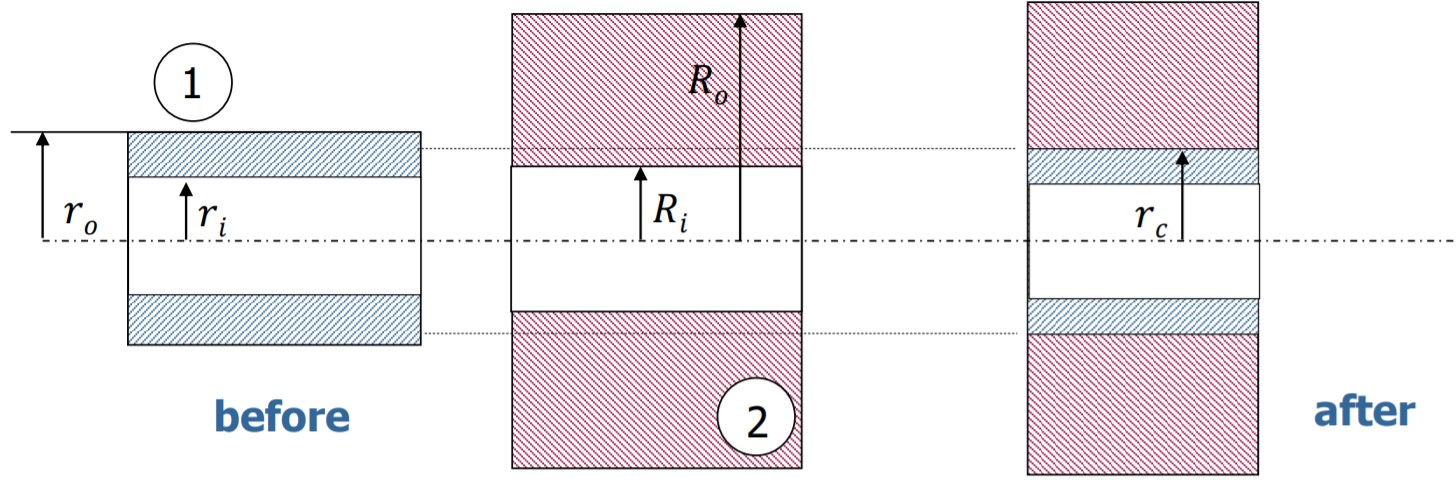
\includegraphics[width=10cm]{interference}
		\caption{dimension of shaft and hub used in the formulas of the press fit.}
	\end{figure}

	\begin{table}[p]
		\centering \rule{0.9\linewidth}{1pt}
		\caption{the first table represent the fundamental deviations for shafts, metric series; size ranges are for "over" the lower limit and "including" the upper one; all values are in $mm$. The second table presents instead the the standard tolerances grades.}
		\label{tab:metricfits}
		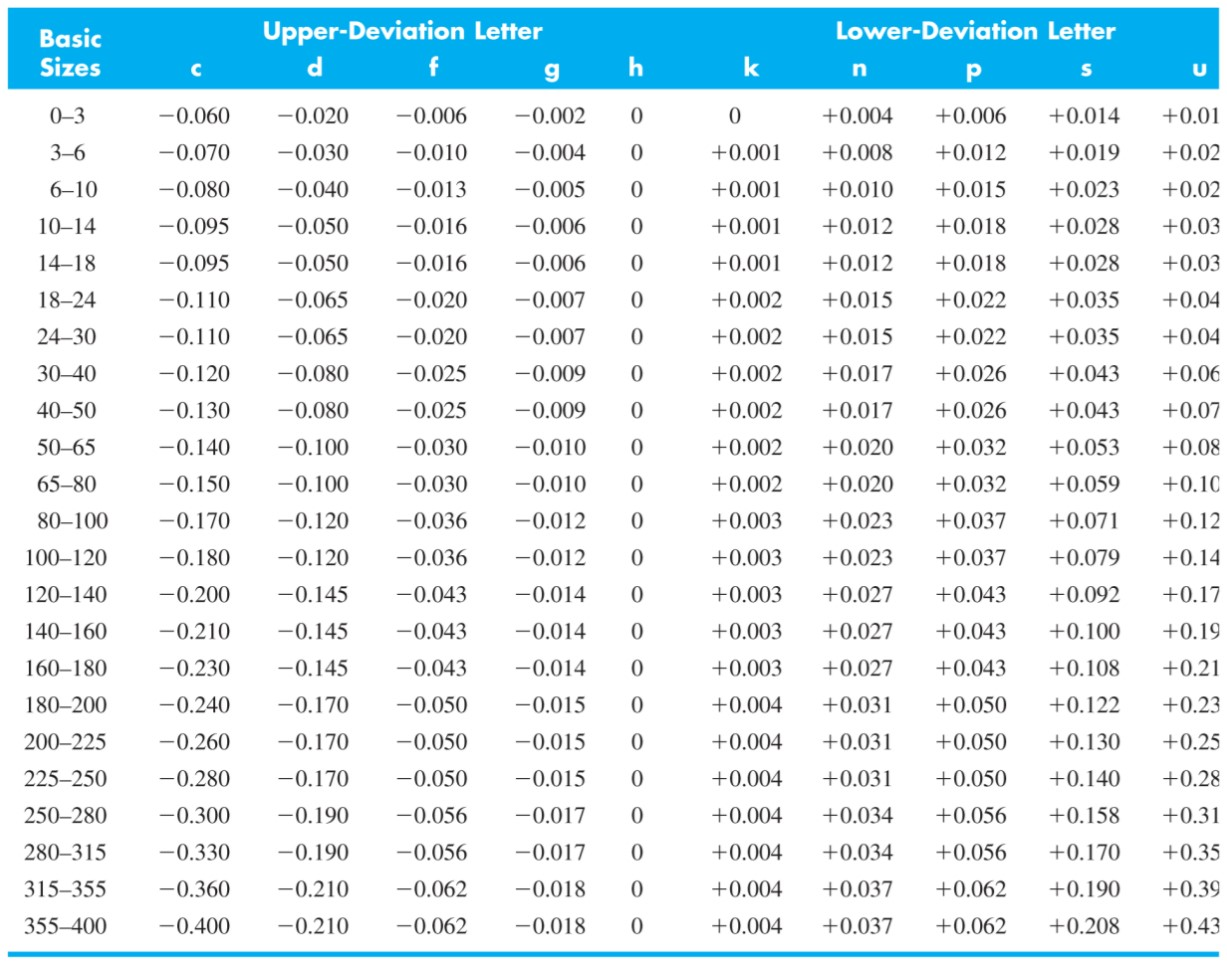
\includegraphics[width=0.95\linewidth]{metricfits}
		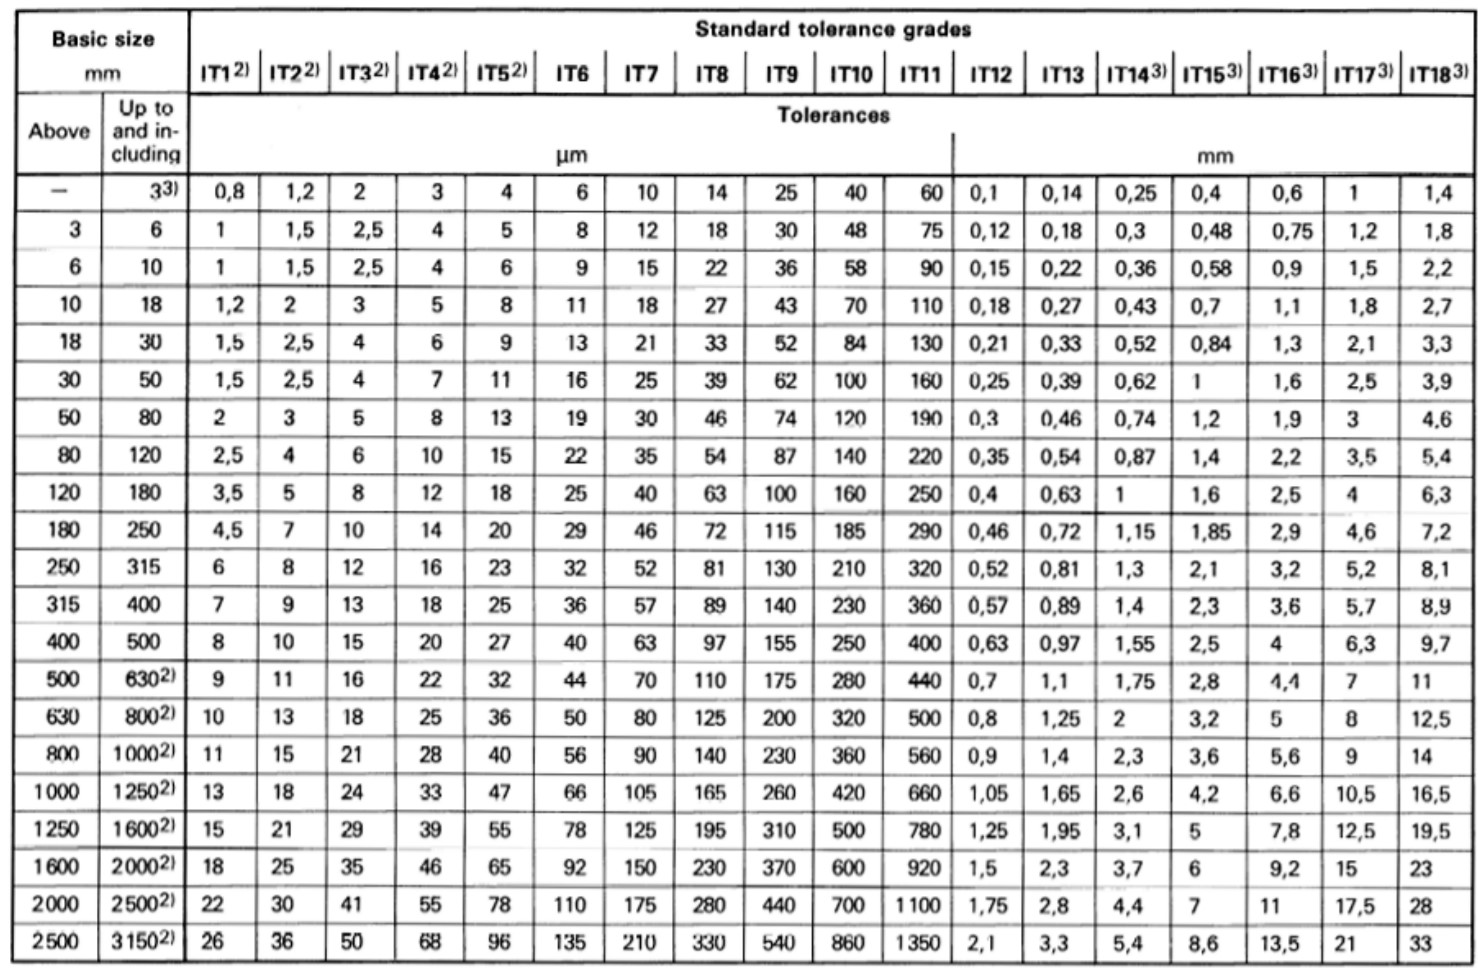
\includegraphics[width=0.95\linewidth]{tolerance-grades}
		\rule{0.9\linewidth}{1pt}
	\end{table}

	Regarding the stress states of a press fit we have to consider the radial and tangential components that on the hub follows the rules
	\begin{equation} \label{eq:pressstress}
		\sigma_r = A - \frac B {r^2} \hspace{3cm} \sigma_\theta = A + \frac B {r^2}
	\end{equation}
	where
	\[ A = \frac{p_i r_i^2 - p_or_o^2}{r_o^2-r_i^2} \hspace{3cm} B = \frac{p_i-p_o}{r_o^2-r_i^2} r_i^2r_o^2 \]
	and $p_i,p_o$ are the boundary conditions for the pressure on the hub. Using the Tresca equivalent stress defined by the law $\seq = |\sigma_r - \sigma_\theta|$ we can note that $\seq = 2 B/r^2$, meaning that for static verification we must check
	\begin{equation} \label{eq:maxinterference}
		2 |p_{c,max}| \frac 1 {1- \frac{r_c^2}{r_o^2}} \leq \frac{\sys}{\phi}
	\end{equation}
	
	
	
	
	
	
	
	
	
	
	
	
	
	
	
	
	
	
	
	
	
	
	
	
	
	
	
	
	
